\documentclass[table]{elegantpaper}
\usepackage{datetime2}
\usepackage[T1]{fontenc}
\usepackage{graphicx}
\usepackage{listings}
\usepackage{listings-rust}
\usepackage{pgf-pie}
\usepackage{rotating}
\usepackage{tabularray}
\usepackage{tabularx}
\usepackage{xcolor}
\usepackage{endnotes}

\DTMusemodule{english}{en-GB}
\DTMnewdatestyle{short}{
  \renewcommand{\DTMdisplaydate}[4]{
    \DTMenglishmonthname{##2} \number##1\relax
  }
  \renewcommand{\DTMDisplaydate}{\DTMdisplaydate}
}
\newcommand{\shorttoday}{{\DTMsetdatestyle{short}\today}}
\renewcommand{\updatetext}{}

\graphicspath{{./images/}}
\DeclareEmphSequence{\bfseries,\itshape,\upshape}
\lstset{xleftmargin=\parindent,xrightmargin=\parindent}

\title{Groth16 Implement Specification in BitVM2}
\author{Fiamma \endnote{\url{https://twitter.com/Fiamma_Chain}}}
\date{\shorttoday}

\addbibresource[location=local]{reference.bib}

\begin{document}
    \maketitle
    \begin{abstract}
    In this paper, we will show how we implement the Groth16 verification in Bitcoin, we are grateful to all the members who contribute to BitVM2 repository,
    such as Robin, Weikeng, and Zerosync team, etc. Based on this paper, we hope:
    (1). Our design and implementment could be reviewed by BitVM2 community;
    (2). Let more developer and researchers to know the details that how BitVM2 works with Groth16;
    (3). Accelerating the process of BitVM2 with whole community to ensure it could be adopted in production in a safe way;
\end{abstract}

    \pagebreak
    \tableofcontents
    \pagebreak
    \section{The Basics} \label{sec:basics}
The section will introduce some basic knowledgers you would better to know, including 
(1). The Groth16 verification progress;
(2). On proving pairing;
(3). Limitations when split the script;

\subsection{Groth16-verification-program}

The verify progress of Groth16\cite{website:Groth16} as follows:

\begin{equation}
0/1 \Leftarrow Vrf(R,\sigma, a_{1},...,a_{l}, \pi): Parse \pi = ([A]_{1}, [C]_{1}, [B]_{2}) \in G_1^2, G_2
\end{equation}

Accept the proof if and only if

\begin{equation}
 [A]_1 \cdot [B]_2 = [\alpha_1] \cdot [\beta]_2 + \sum_{0}^{l}a_i[\frac{\beta\mu_i(x) + \alpha\upsilon_i(x) + \omega_i(x)}{\gamma}]_1 \cdot [\gamma]_2 + [C]_1 \cdot [\delta]_2  
\end{equation}


Let \begin{equation}  [msm]_1 = \sum_{0}^{l}a_i[\frac{\beta\mu_i(x) + \alpha\upsilon_i(x) + \omega_i(x)}{\gamma}]_1 \end{equation}



It should be noted that $a_0 = 1$ 

\subsection{On-proving-pairing}

This is a efficient ways to prove correctness of \cite{website:On-proving-pairing}, the algorithm shows in page 25:

Algorithm 9: Multi Miller loop with embedded $c$ exponentiation 

Input: $\displaystyle A = [(P_1,Q_1), (P_2,Q_2),...,(P_n,Q_n)],c, c^{-1} \in F_{q^k},s \in F_{q^3},P_{Q_j} \leftarrow \mathcal{L}(Q_j)$ 

Output: $\displaystyle 1 \ \ if \prod_{i=0}^{n}e(P_i, Q_i) = 1 $ 

(1) assert $\displaystyle c \cdot c^{-1} = 1 $ 

(2) $\displaystyle f \leftarrow c^(-1), lc \leftarrow 0 $ 

(3) Initialize array $T$ such that $\displaystyle T[j] = Q_j $ for each non-fixed point $Q_j$ 

(4) for $i$ = $L-2$ to $0$ do 

(5) \indent $f$ = $f^2$ 

(6) \indent for j=1 to n do 

(7) \indent \indent $\displaystyle l \leftarrow P_{Q_j}[lc] $ 

(8) \indent \indent $\displaystyle f = f \cdot l.evaluate(P_j) $  

(9) \indent \indent if $Q_j$ is not fixed then 

(10) \indent \indent \indent $\displaystyle T \leftarrow T[j] $ 

(11) \indent \indent \indent assert $\displaystyle l.is_tangent(T) $ 

(12) \indent \indent \indent $\displaystyle T[j] = l.double(T) $ 

(13) \indent \indent end 

(14) \indent \indent if $bit^2 == 1$ then 

(15) \indent \indent \indent $\displaystyle f = f \cdot c^{-1}$ if $bit$ == 1 else $\displaystyle f \cdot c$ end 

(16) \indent \indent \indent $\displaystyle l \leftarrow P_{Q_j}[lc+1] $ 

(17) \indent \indent \indent $\displaystyle f = f \cdot l.evaluate(P_{j})$ 

(18) \indent \indent \indent if $Q_j$ is not fixed then 

(19) \indent \indent \indent \indent $\displaystyle Q^{'} = Q_j $ if $bit$ == 1 else $\displaystyle -Q_j $ 

(20) \indent \indent \indent $\displaystyle T \leftarrow T[j] $ 

(21) \indent \indent \indent assert $\displaystyle l.is_line(T, Q^{'}) $ 

(22) \indent \indent \indent $\displaystyle T[j] = l.add(T, Q^{'}) $ 

(23) \indent \indent \indent end 

(24) \indent \indent end 

(25) \indent end 

(26) \indent $\displaystyle lc = lc + 2 $ 

(27) \indent for j=0 to n do 

(28) \indent \indent $\displaystyle f \leftarrow f \cdot s \cdot (c^{-1})^q \cdot (c^{-1})^{q^2} \cdot (c^{-1})^{q^3} $ 

(29) \indent \indent $\displaystyle l_{1..3} \leftarrow (P_{Q_j}[lc+i])_{i=0}^2 $ 

(30) \indent \indent $\displaystyle f \leftarrow f \cdot l_1.evaluate(P_{j}) \cdot l_2.evaluate(P_{j}) \cdot l_3.evaluate(P_{j}) $ 

(31) \indent \indent if $Q_j$ is not fixed then 

(32) \indent \indent \indent $\displaystyle Q_1 \leftarrow \pi_p(Q), Q_12\leftarrow \pi_p(Q_1), Q_3 \leftarrow \pi_p(Q_2) $ 

(33) \indent \indent \indent $\displaystyle T \leftarrow T[j] $ 

(34) \indent \indent \indent assert $\displaystyle l_1.is_line(T, Q_1); T \leftarrow T + Q_1 $ 

(35) \indent \indent \indent assert $\displaystyle l_2.is_line(T, -Q_2); T \leftarrow T - Q_1 $ 

(36) \indent \indent \indent assert $\displaystyle l_3.is_line(T, Q_3) $ 

(37) \indent \indent end 

(38) \indent end 

(39) end 

(40) return $\displaystyle f == 1? $ 


if We adopt this algorithm into Groth16, The whole algorithm process should be like this:

$\displaystyle P_1 = [msm]_1; Q_1 = -[\gamma]_2 $

$\displaystyle P_2 = [C]_1; Q_2 = -[\delta]_2 $

$\displaystyle P_3 = [\alpha]_1; Q_3 = -[\beta]_2 $

$\displaystyle P_4 = [A]_1; Q_4 = [B]_2 $


$Q_4$ is non-fixed, $Q_1$, $Q_2$, and $Q_3$ is fixed.


Input: $\displaystyle A = [(P_1,Q_1), (P_2,Q_2), (P_3,Q_3),(P_4,Q_4)],c, c^{-1} \in F_{q^k},s \in F_{q^3},P_{Q_4} \leftarrow \mathcal{L}(Q_4)$ 

Output: $\displaystyle 1 \ \ if \prod_{i=0}^{n}e(P_i, Q_i) = 1 $ 

(1) assert $\displaystyle c \cdot c^{-1} = 1 $ 

(2) $\displaystyle f \leftarrow c^(-1), lc \leftarrow 0 $ 

(3) Initialize array $T$ such that $\displaystyle T[j] = Q_j $ for each non-fixed point $Q_j$ 

(4) for $i$ = $L-2$ to $0$ do 

(5) \indent $f$ = $f^2$ 

(6) \indent \indent $\displaystyle f = f \cdot c^{-1}$ if $bit$ == 1 else $\displaystyle f \cdot c$ end 

(7) \indent for j = 1 to 4 do 

(7) \indent \indent $\displaystyle l \leftarrow P_{Q_j}[lc] $ 

(8) \indent \indent $\displaystyle f = f \cdot l.evaluate(P_j) $  

(8) \indent end 

(9) \indent $Q_4$ is not fixed then 

(8) \indent $\displaystyle f = f \cdot l.evaluate(P_4) $  

(10) \indent $\displaystyle T \leftarrow T[j] $ 

(11) \indent assert $\displaystyle l.is_tangent(T) $ 

(12) \indent $\displaystyle T[j] = l.double(T) $ 

(14) \indent if $bit == 1$ or $bit == -1 $ then 

(7) \indent \indent for j = 1 to 4 do 

(7) \indent \indent \indent $\displaystyle l \leftarrow P_{Q_j}[lc + 1] $ 

(8) \indent \indent \indent $\displaystyle f = f \cdot l.evaluate(P_j) $  

(8) \indent \indent end 

(18) \indent \indent $Q_4$ is not fixed then 

(16) \indent \indent  $\displaystyle l \leftarrow P_{Q_j}[lc+1] $ 

(17) \indent \indent  $\displaystyle f = f \cdot l.evaluate(P_{j})$ 

(19) \indent \indent  $\displaystyle Q^{'} = Q_j $ if $bit$ == 1 else $\displaystyle -Q_j $ 

(20) \indent \indent  $\displaystyle T \leftarrow T[j] $ 

(21) \indent \indent  assert $\displaystyle l.is_line(T, Q^{'}) $ 

(22) \indent \indent  $\displaystyle T[j] = l.add(T, Q^{'}) $ 

(24) \indent  end 

(28) \indent  $\displaystyle f \leftarrow f \cdot s \cdot (c^{-1})^q \cdot c^{q^2} $ 

(7) \indent \indent for j = 1 to 4 do 

(30) \indent \indent $\displaystyle f \leftarrow f \cdot l_1.evaluate(P_{j}) $ 

(7) \indent \indent end 

(31) \indent \indent $Q_4$ is not fixed then 

(32) \indent \indent  $\displaystyle Q_1 \leftarrow \pi_p(Q), Q_12\leftarrow \pi_p(Q_1), Q_3 \leftarrow \pi_p(Q_2) $ 

(33) \indent \indent  $\displaystyle T \leftarrow T[j] $ 

(34) \indent \indent  assert $\displaystyle l_1.is_line(T, Q_1); T \leftarrow T + Q_1 $ 

(35) \indent \indent  assert $\displaystyle l_2.is_line(T, -Q_2); T \leftarrow T - Q_1 $ 

(36) \indent \indent  assert $\displaystyle l_3.is_line(T, Q_3) $ 

(38) \indent end 

(39) end 

(40) return $\displaystyle f == 1? $ 
\subsection{Limitations-on-bitcoin-script}

Several constraints must be considered:
\begin{itemize}
    \item Max script size: 4MB
    \item Max stack depth: 1000 (combined main stack and alternate stack);
    \item Max signatures number in one block: 1000 Winternitz signatures;
\end{itemize}

\subsection{Block-size-calculation}

It would be better know that how we calculate the Bitcoin block size based on taproot upgrade now.

\subsubsection{block size}

The block size will be calculated as the following picture:

\begin{figure}[ht] 
    \centering  
    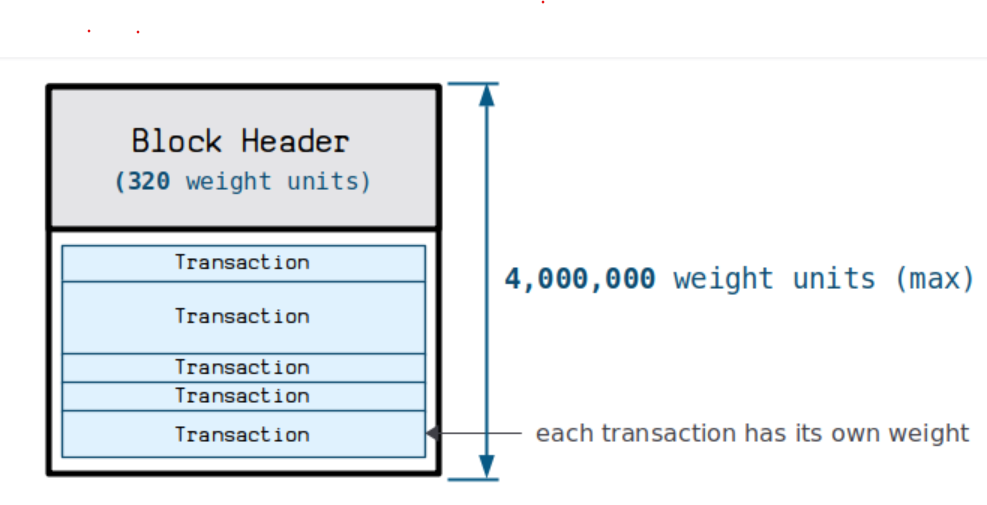
\includegraphics[width=0.85\columnwidth]{images/block-size.png} 
    \caption{Block size}
    \label{fig:block-size}
\end{figure}

\subsubsection{transaction size}

The transaction size will be calculated as the following picture:

\begin{figure}[ht] 
    \centering  
    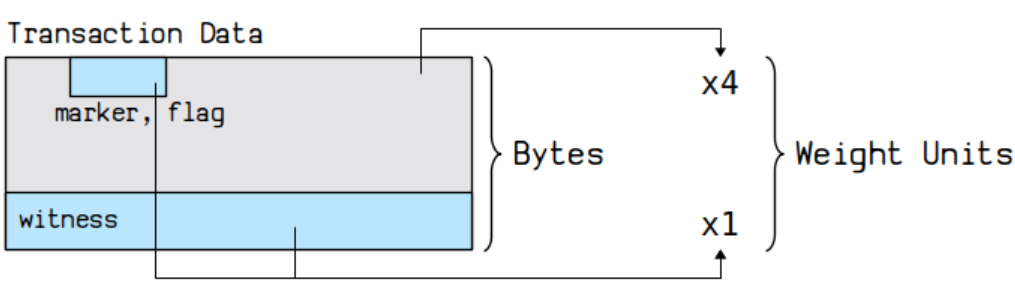
\includegraphics[width=0.85\columnwidth]{images/transaction-size.png} 
    \caption{Transaction size}
    \label{fig:transaction-size}
\end{figure}

You can check more details in \cite{website:transaction-size}

\subsubsection{script chunk limitation}

Based on the deign of BitVM2 \cite{website:BitVM2}, we hope each script chunk could be packed into one block as a transaction.
So, the transaction size could not exceed 4,000,000 - 320 = 3,999,680 weight units \cite{website:transaction-size}.

The disputed transaction is a 1 input and 2 outputs, the average size of non-witness data in this kind of transaction is around 464 weight units.
So for the witness size, the limitation is 3,999,680 - 464 = 3,999,216 weight units.

As showed in BitVM2 \cite{website:BitVM2}, the disputed transaction needs to the signature of Committee, and the sign type is
SIGNHASH\_SINGLE. Let's assume that the number of Committee is 7 and the size of each schnorr signature is 65 bytes (64 bytes for SIGNHASH\_ALL)

So the limitation will be 3,999,216 - 7 * 75 - 8(stack item size) = 3,998,683 weight units.

\begin{figure}[ht] 
    \centering  
    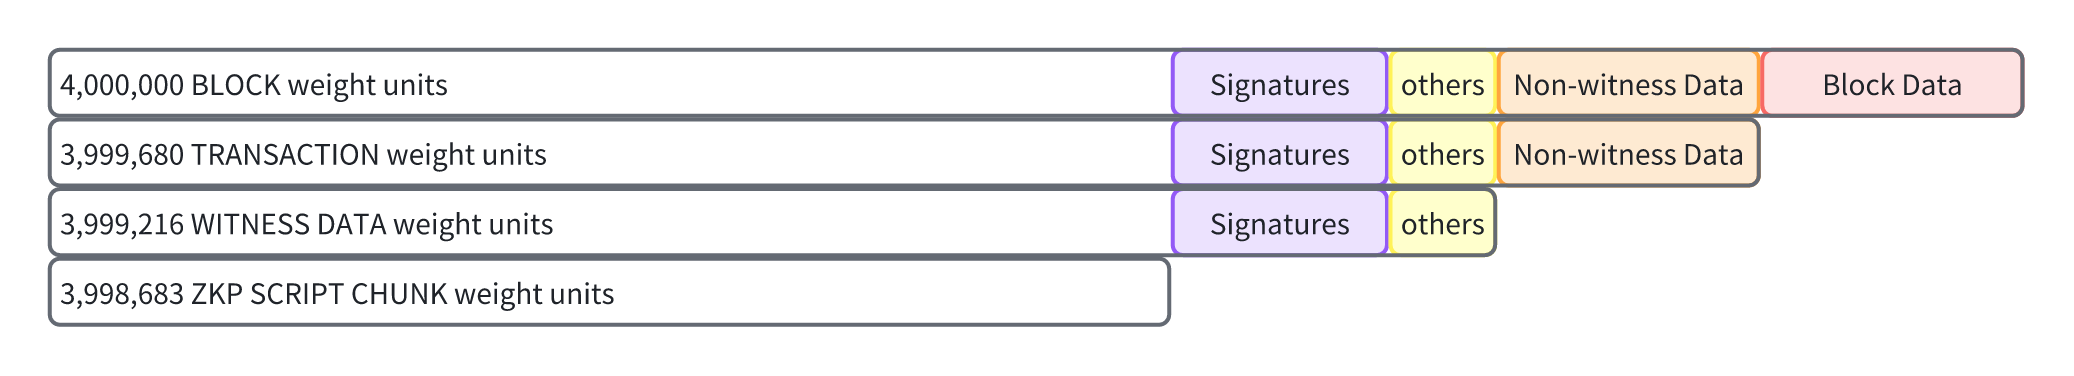
\includegraphics[width=0.85\columnwidth]{images/ZKP-script-chunk-limitation.png} 
    \caption{ZKP script chunk limitation}
    \label{fig:ZKP-script-chunk-limitation}
\end{figure}


\subsection{Transaction constructure}

The transaction constructure of Bitcoin show in the following excel.

\begin{tabular}{|c|c|c|} \hline
    Field & Size & Description \\ \hline
    Version & 4 bytes & The version number for the transaction. Used to enable new features  \\ \hline
    \textcolor{blue}{Maker} & 1 bytes & Used to indicate a segwit transaction. Must be 00 \\ \hline
    \textcolor{blue}{Flag} & 1 bytes & Used to indicate a segwit transaction. Must be 01 or greater  \\ \hline
    Input Count & Variable & Indicates the number of inputs  \\ \hline
    Input-TXID & 32 bytes & The TXID of the transaction containing the output you want to spend  \\ \hline
    Input-VOUT & 4 bytes & The index number of the output you want to spend  \\ \hline
    Input-ScriptSig Size & Variable & The size in bytes of the upcoming ScriptSig  \\ \hline
    Input-ScriptSig & Variable & The unlocking code for the output you want to spend  \\ \hline
    Input-Sequnencer & 4 bytes & Set whether the transaction can be replaced or when it can be mined  \\ \hline
    Output Count & Variable & Indicates the number of outputs  \\ \hline
    Output-Amount & 8 bytes & The value of the output in satoshis  \\ \hline
    Output-ScriptPubKey Size & Variable & The size in bytes of the upcoming ScriptPubKey  \\ \hline
    Output-ScriptPubKey & Variable bytes & The locking code for this output  \\ \hline
    \textcolor{blue}{Witness-Stack Items} & Variable & The number of items to be pushed on to the stack as part of the unlocking code.  \\ \hline
    \textcolor{blue}{Witness-Stack Items-Size} & Variable & The size of the upcoming stack item  \\ \hline
    \textcolor{blue}{Witness-Stack Items-Item} & Variable & The data to be pushed on to the stack  \\ \hline
    Locktime & 4 bytes & Set a time or height after which the transaction can be mined  \\ \hline
\end{tabular}

The \textcolor{blue}{blue} part means it will be stored in segwit part. Any one could check more details in \cite{website:transaction-constructure}
\subsection{Signature-hash-type}


Signature Hash Types:

0x01 = SIGHASH\_ALL
0x02 = SIGHASH\_NONE
0x03 = SIGHASH\_SINGLE
0x81 = SIGHASH\_ANYONECANPAY | SIGHASH\_ALL
0x82 = SIGHASH\_ANYONECANPAY | SIGHASH\_NONE
0x83 = SIGHASH\_ANYONECANPAY | SIGHASH\_SINGLE
    \subsection{Bench data} \label{sec:bench-data}

This section mainly give some bench datas for some operators used in Groth16 verification process.

\subsubsection{Operators script size origin}

We will first present some initial benchmark data from our current implementation, including:

\begin{itemize}
    \item Double and Add operators in $G_1$ group;
    \item Double and Add operators in $G_2$ group;
    \item Field operators in extension field;
\end{itemize}

\paragraph*{G1 group}

\begin{center}
\begin{tabular}{|c|c|c|c|} \hline
operator type & script size & max depth & exceed 4M? \\ \hline
$2 \cdot g_1$ & 1,752,916 bytes & 131 & no  \\ \hline
$g_1 \cdot g_1^{'}$ & 3,997,319 bytes &	< 1000 & no \\ \hline
\end{tabular}
\end{center}

\paragraph*{G2 group}

\begin{center}
\begin{tabular}{|c|c|c|c|} \hline
operator type & script size & max depth & exceed 4M? \\ \hline
$2 \cdot g_2$ & \textcolor{red}{7,019891} bytes & 815 & yes  \\ \hline
$g_2 \cdot g_2^{'}$ & \textcolor{red}{9,270,854} bytes &	293 & yes \\ \hline
\end{tabular}
\end{center}

\paragraph*{field}

\begin{center}
\begin{tabular}{|c|c|c|c|} \hline
operator type & script size & max depth & exceed 4M? \\ \hline
$F_{q12}: a + b$ & 6,644 bytes & 220 & no  \\ \hline
$F_{q12}: 2 * a$ & 6,793 bytes & 217 & no \\ \hline
$F_{q12}: a * b$ & \textcolor{red}{11,641,775} bytes & 545 & yes \\ \hline
$F_{q12}: a * a$ & \textcolor{red}{7,772,080} bytes & 545 & yes \\ \hline
$F_{q12}: mul\_fq6\_by\_nonresidue$ & 4,923 bytes &	146 & no \\ \hline
$F_{q12}: frobenius\_map(1)$ & \textcolor{red}{4,541,887} bytes & - & yes \\ \hline
$F_{q12}: frobenius\_map(2)$ & 2,224,363 bytes & - & yes \\ \hline
$F_{q12}: mul\_by\_034$ & \textcolor{red}{9,810,459} bytes &	- & yes \\ \hline
$F_{q12}: ell\_by\_constant$ & \textcolor{red}{9,525,050} bytes & 383 & yes \\ \hline
$F_{q6}: a * b$ & 3,873,847 bytes &	275 & no \\ \hline
$F_{q6}: frobenius\_map(1)$ & 1,518,206 bytes &	- & no \\ \hline
$F_{q6}: frobenius\_map(2)$ & 598,274 bytes & - & no \\ \hline
$F_{q6}: mul\_by\_01\_with\_1\_constant$ & 3,280,529 bytes & 221 & no \\ \hline
$F_{q6}: mul\_by\_fp2\_constant$ & 1,520,337 bytes & 101 & no \\ \hline
$F_{q6}: mul\_by\_01$ & 3,769,633 bytes & - & no \\ \hline
$F_{q6}: mul\_by\_fp2$ & 2,252,362 bytes &	167 & no \\ \hline
$F_{q2}: a * b$ & 750,883 bytes & 113 & no \\ \hline

\end{tabular}
\end{center}

\subsubsection{Operator script size optimization}

The fewer script chunks, the better. Therefore, before we split the large operators, we aim to optimize them first. We will present our new 
data initially, followed by an explanation of the principle.

\begin{itemize}
    \item Double and Add operators in $G_1$ group;
    \item Double and Add operators in $G_2$ group;
    \item Field operators in extension field;
\end{itemize}

\paragraph*{G1 group}

\begin{center}
\begin{tabular}{|c|c|c|c|} \hline
operator type & script size & optimized script size & exceed 4M? \\ \hline
$2 \cdot g_1$ & 1,752,916 bytes & \textcolor{green}{699,519} bytes & no  \\ \hline
$g_1 \cdot g_1^{'}$ & 3,997,319 bytes &	\textcolor{green}{562,445} bytes & no \\ \hline
\end{tabular}
\end{center}

\paragraph*{G2 group}

\begin{center}
\begin{tabular}{|c|c|c|c|} \hline
operator type & script size & optimized script size & exceed 4M? \\ \hline
$2 \cdot g_2$ & \textcolor{red}{7,019,891} bytes & \textcolor{green}{1,847,059} bytes & yes  \\ \hline
$g_2 \cdot g_2^{'}$ & \textcolor{red}{9,270,854} bytes & \textcolor{green}{1,563,501} bytes & yes \\ \hline
\end{tabular}
\end{center}

\paragraph*{Field}

\begin{center}
\begin{tabular}{|c|c|c|c|} \hline
operator type & script size & optimized script size & exceed 4M? \\ \hline
$F_{q12}: a + b$ & 6,644 bytes & 6,644 bytes & no  \\ \hline
$F_{q12}: 2 * a$ & 6,793 bytes & 6,793 bytes & no \\ \hline
$F_{q12}: a * b$ & \textcolor{red}{11,641,775} bytes & \textcolor{green}{\textbf{6,727,971}} bytes & yes \\ \hline
$F_{q12}: a * a$ & \textcolor{red}{7,772,080} bytes & \textcolor{green}{\textbf{4,495,790}} bytes & yes \\ \hline
$F_{q12}: mul\_fq6\_by\_nonresidue$ & 4,923 bytes & 4,923 bytes & no \\ \hline
$F_{q12}: frobenius\_map(1)$ & \textcolor{red}{4,541,887} bytes & \textcolor{green}{2,879,118} bytes & no \\ \hline
$F_{q12}: frobenius\_map(2)$ & 2,224,363 bytes & \textcolor{red}{2,791,858} bytes  & no \\ \hline
$F_{q12}: mul\_by\_034$ & \textcolor{red}{9,810,459} bytes & \textcolor{green}{\textbf{4,289,505}} bytes & yes \\ \hline
$F_{q12}: ell\_by\_constant$ & \textcolor{red}{9,525,050} bytes & \textcolor{green}{\textbf{4,714,973}} bytes  & yes \\ \hline
$F_{q6}: a * b$ & 3,873,847 bytes & \textcolor{green}{2,236,303} bytes & no \\ \hline
$F_{q6}: frobenius\_map(1)$ & 1,518,206 bytes & \textcolor{green}{933,606} bytes & no \\ \hline
$F_{q6}: frobenius\_map(2)$ & 598,274 bytes & \textcolor{red}{958,404} bytes & no \\ \hline
$F_{q6}: mul\_by\_01\_with\_1\_constant$ & 3,280,529 bytes & \textcolor{green}{1,925,215} bytes & no \\ \hline
$F_{q6}: mul\_by\_fp2\_constant$ &  1,520,337 bytes & \textcolor{green}{960,147} bytes & no \\ \hline
$F_{q6}: mul\_by\_01$ & 3,769,633 bytes & \textcolor{green}{2,136,209} bytes & no \\ \hline
$F_{q6}: mul\_by\_fp2$ & 2,252,362 bytes & \textcolor{green}{1,273,623} bytes & no \\ \hline
$F_{q2}: a * b$ & 750,883 bytes & \textcolor{green}{424,433} bytes & no \\ \hline

\end{tabular}
\end{center}


    \subsection{Split principle} \label{sec:split-principle}

In this section, we will primarily discuss why we choose a manual method for splitting the ZKP verification script.

\subsubsection{Automated}

Automating the splitting of the entire computation is appealing. Ideally, the whole process shoule be similar to the following figure:

\begin{figure}[ht] 
    \centering  
    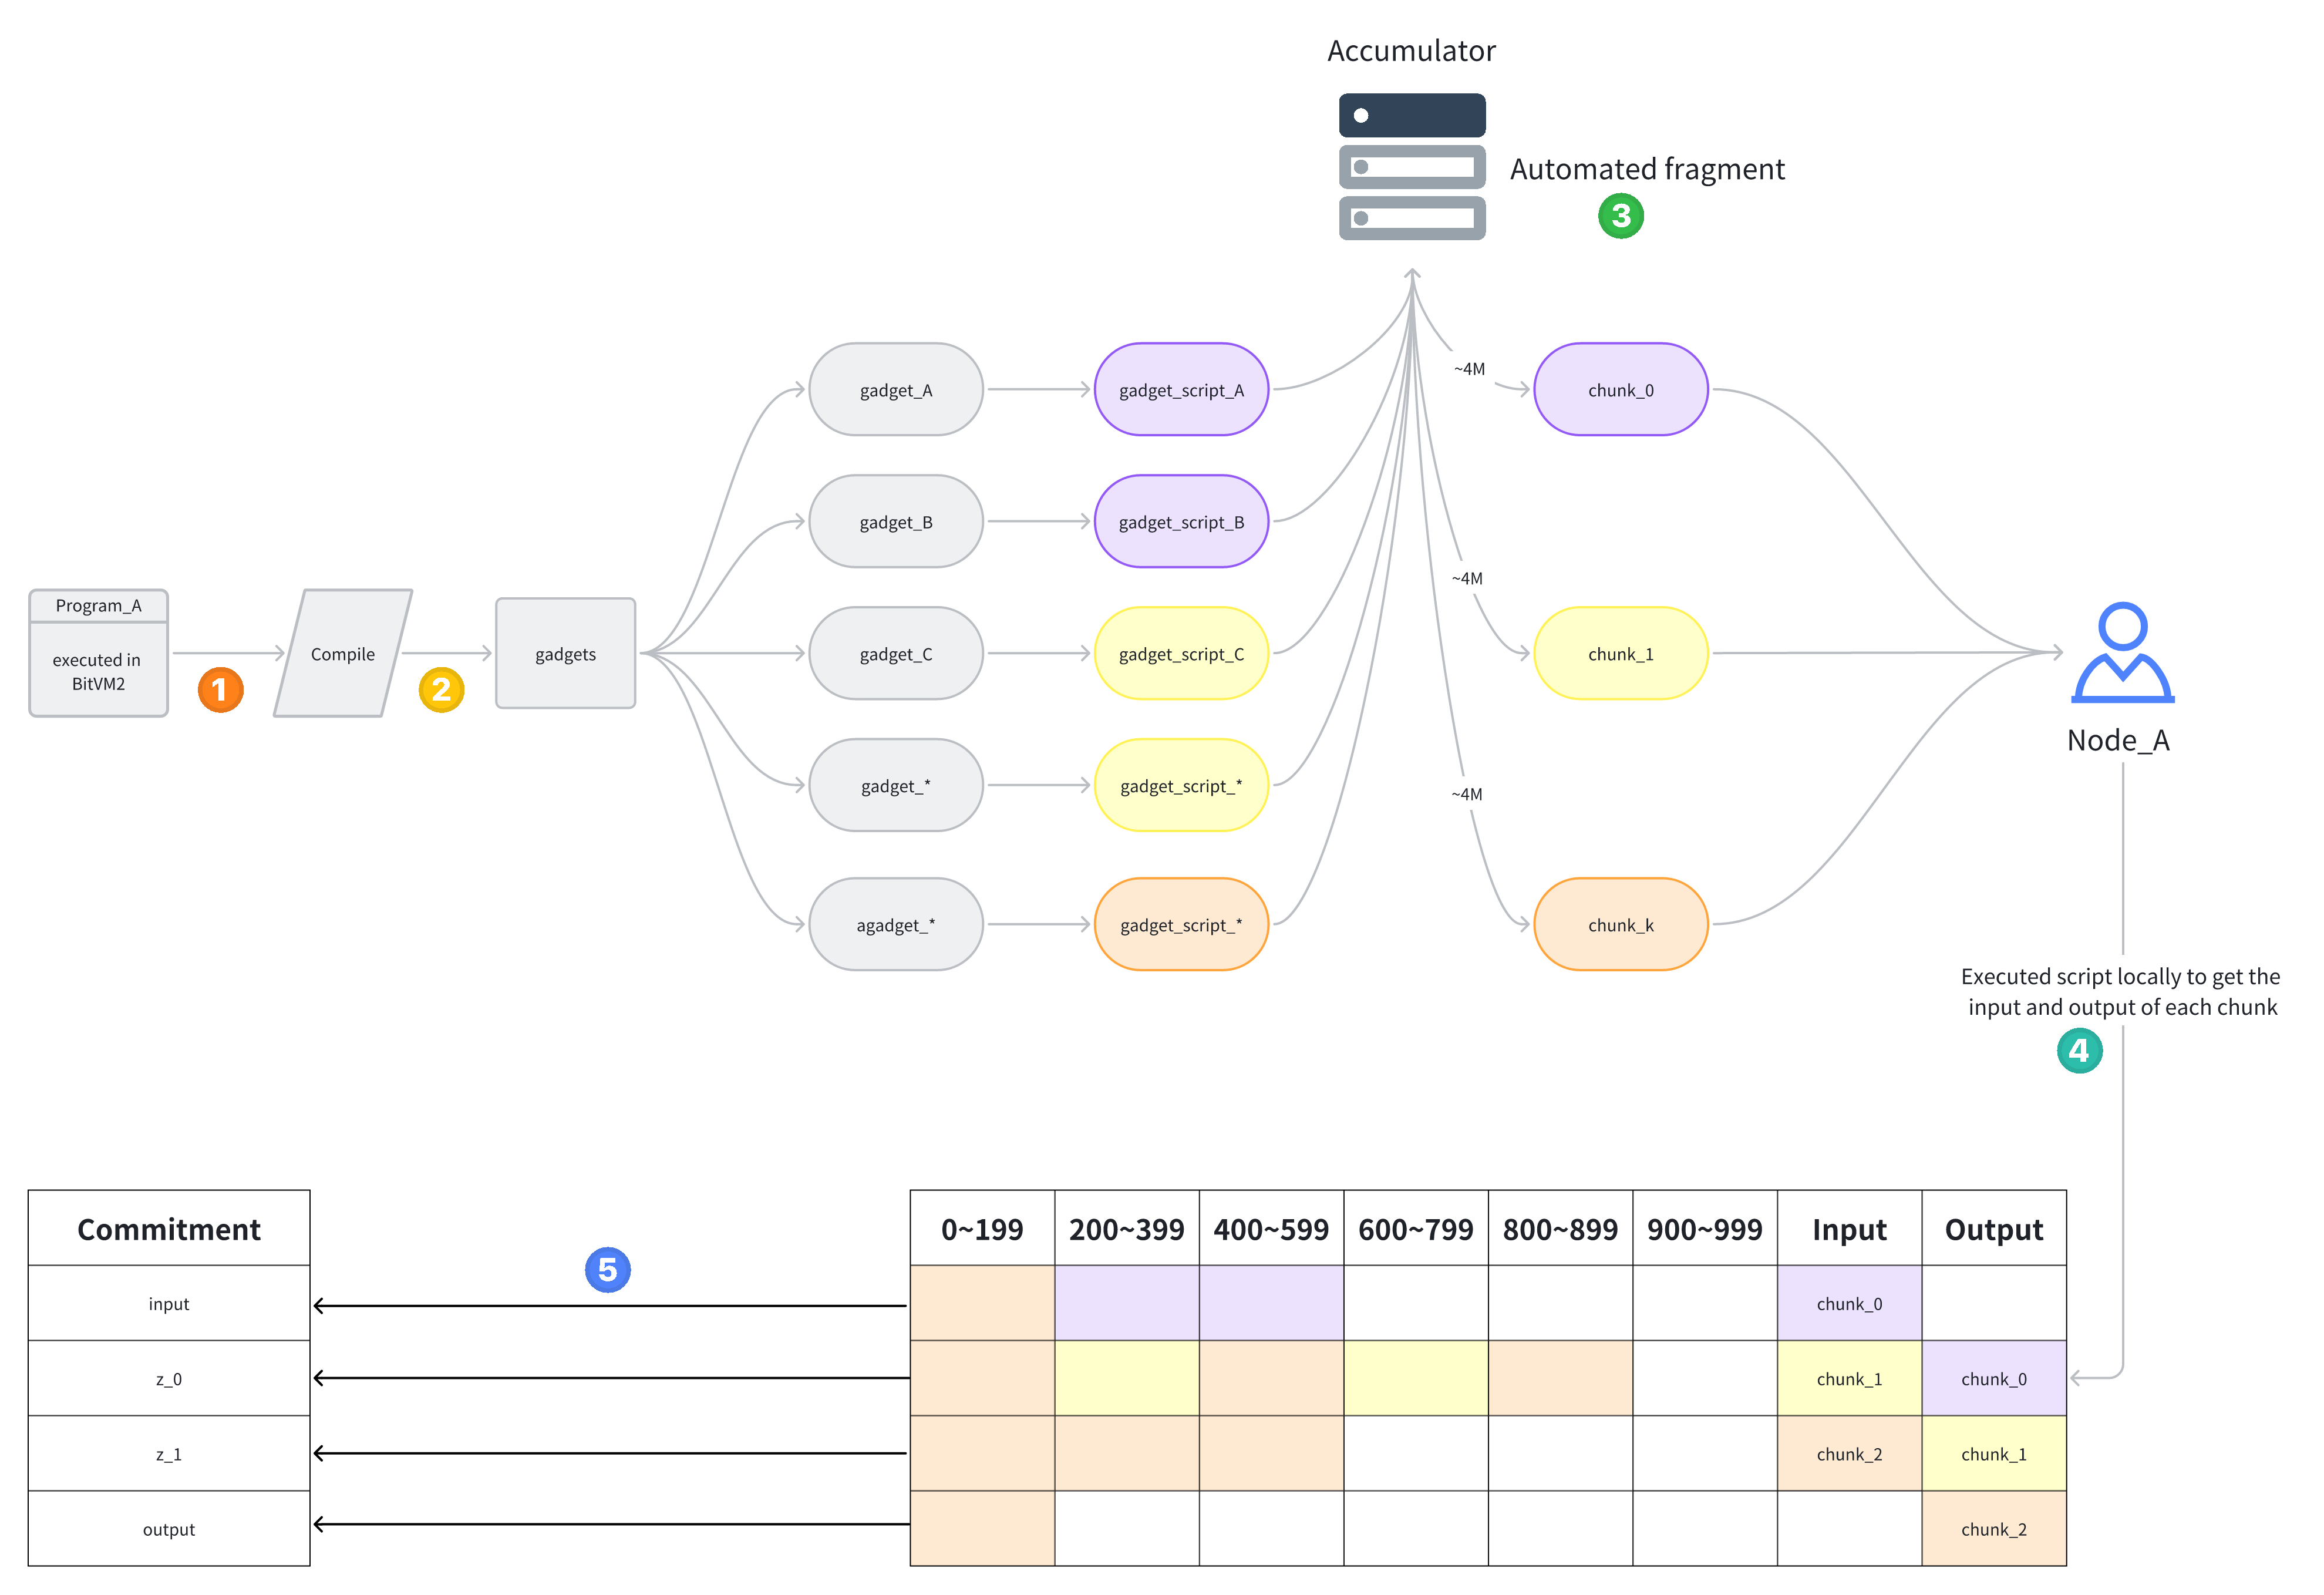
\includegraphics[width=0.85\columnwidth]{images/automated-fragment.png} 
    \caption{automated fragment}
    \label{fig:automated-fragment}
\end{figure}

The overall flow shoule be as follows:
\begin{itemize}
    \item The program will be complied into a set of customized gadgets first;
    \item Each gadget will correspond with a script gadget;
    \item The accmulator will begin to split all gadgets;
    \item Becasue each script gadget has a fixed size, these gadgets will be spilt as one chunk when their accumulated size is almost equal to 4M;
    \item Node A executes the script program locally to generate input and output for each chunk;
    \item All the input and output locate in stack, so Node A has to commit all the value in the stack;
\end{itemize}

It is important to note that stack depth is another factor that should be considered. In the automated approach, there are several constraints:
\begin{itemize}
    \item It is easy to exceed the stack depth limitation;
    \item It commits many values which will not be used in the current chunk;
    \item It must implememnt enough gadgets to support any computation, which means achieving turing completeness;
    \item Executing a large scirpt program is much slower;
    \item It increases the costs when verifying the expected input and output on-chain;
    \item The logic of each chunk is unreadable;
\end{itemize}

However, automated fragmentation has its advantages as well, such as generating the minimal number of script chunks. 
But since we do not upload all chunks to the Bitcoin network, the number of chunks is less of a concern unless their size becomes excessively large.

\subsubsection{Manual}

Why do we adopt a manual way to split the entire program?

\begin{itemize}
    \item We avoid exceeding the stack depth limitation by only placing necessary data for the current chunk on the stack;
    \item We commit only the data used in the current chunk;
    \item We just need to implement gadgets to support ZKP verification as any computaion could generate a ZK proof;
    \item We use a Rust program to generate the input and output for each chunk;
    \item This approach minimizes costs when verifying the expected input and output on-chain;
    \item The logic of each chunk is readable.
\end{itemize}

\begin{figure}[ht] 
    \centering  
    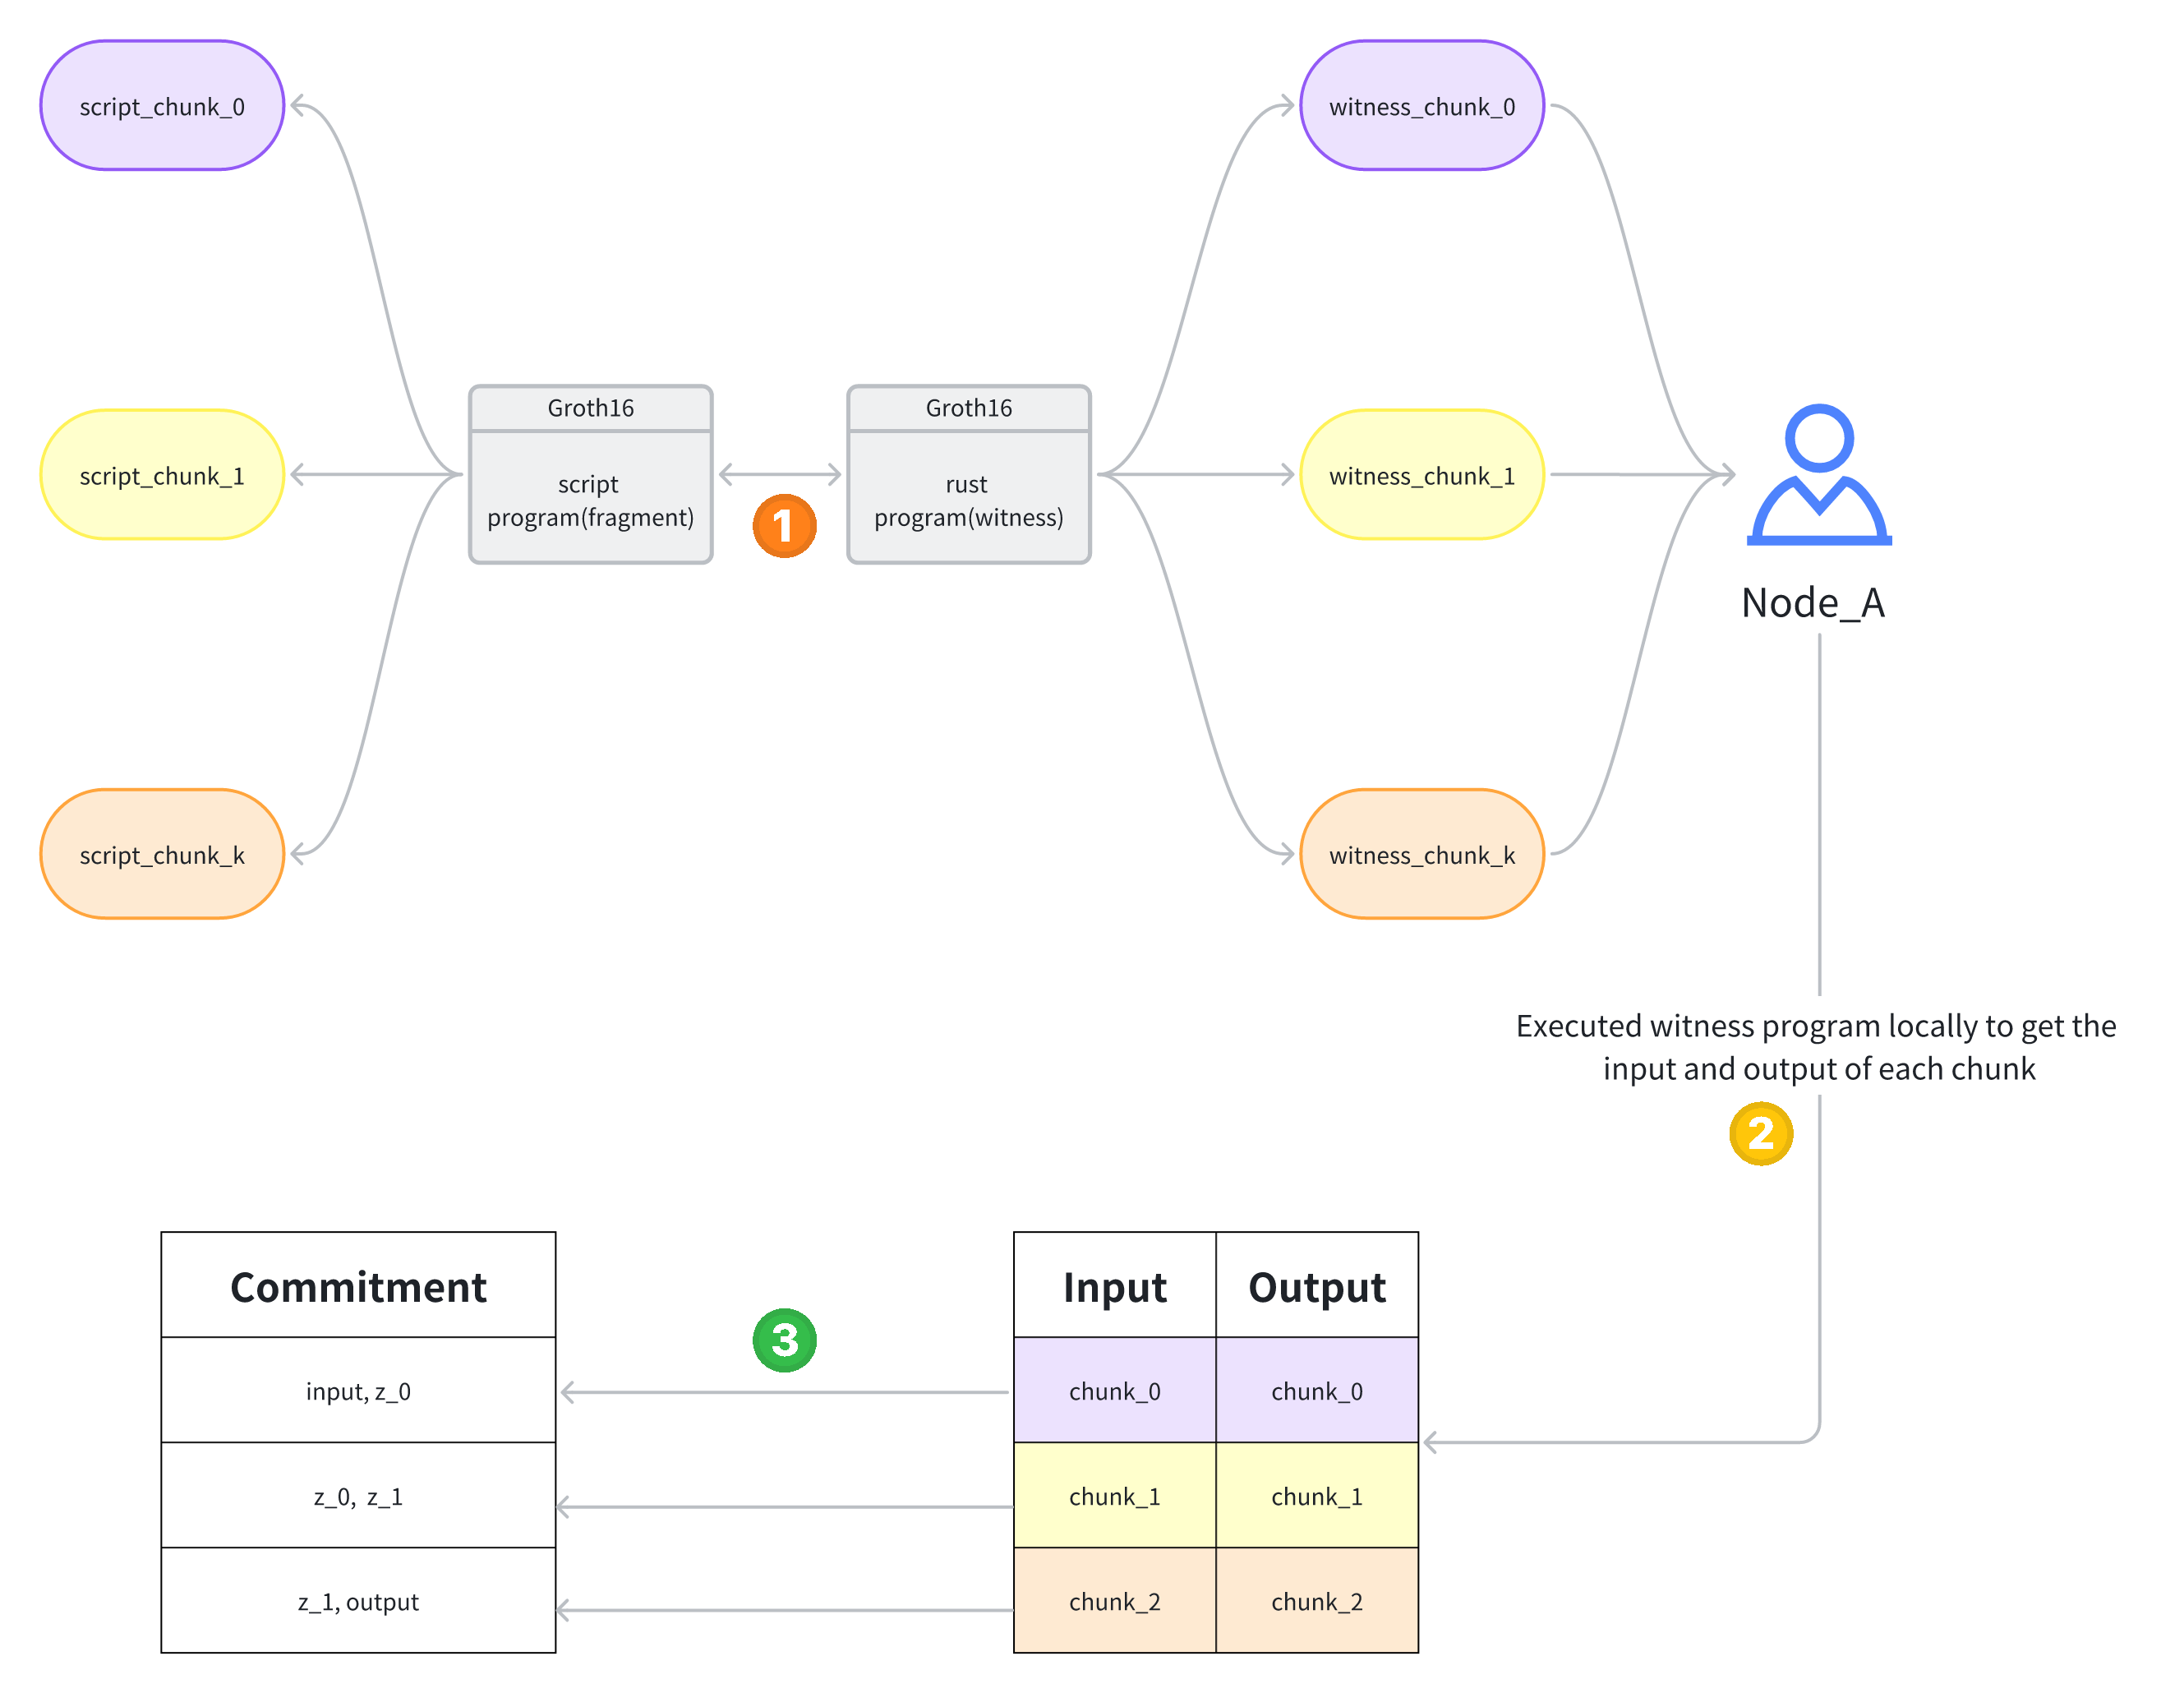
\includegraphics[width=0.65\columnwidth]{images/manually-fragment.png} 
    \caption{manual fragmentation}
    \label{fig:manually-fragment}
\end{figure}

While this approach may generate more chunks, as mentioned earlier, only one script chunk is executed on Bitcoin, so this is acceptable. The overall flow proceeds as follows:
\begin{itemize}
    \item We first concurrently implement the Rust and script versions of the Groth16 ZKP verification;
    \item The rust version includes the witness generation of each chunk;
    \item The script version includes all split chunks;
    \item We ensure each chunk meets the size and depth constraints;
    \item Node A executes the Rust program locally to generate inputs and outputs for each chunk;
    \item Node A commits all the inputs and outputs.
\end{itemize}


    \section{Optimization pricinple} \label{sec:optimization-pricinple}

We will mainly introduce how we recude the script of operators in $G_1$ and $G_2$.

\subsection{group-g1}

It needs more opcodes if we implement the double or add operator in $G_1$ directly because there are some divison operators which
is not bitcoin-friendly. We obey the rules proposed in paper On Proving pairing.


\subsubsection{Double}

\begin{itemize}
    \item Show that the pair ($\lambda$, $\mu$), indeed define a tangent through $T$ showing that $\displaystyle y_1 - \lambda x_{1} - mu = 0$ 
    and $\displaystyle 2\lambda y_1 = 3x_1^2$. This step is dominated by $2\tilde{m}$ and one $\tilde{s}$
    \item Compute $\lambda^2$ which is simple one $\tilde{s}$
    \item Compute $\displaystyle x_3 = \lambda^2-2x_1$ and $\displaystyle 2\lambda y_3 = -\mu - \lambda x_3$ which is dominated by computing $\lambda x_3$
\end{itemize}

\subsubsection{Add}

\begin{itemize}
    \item Show that the pair ($\lambda$, $\mu$), indeed define a tangent through $T$ showing that $\displaystyle y_1 - \lambda x_{1} - mu = 0$ 
    and $\displaystyle y_2 - \lambda x_{2} - mu = 0$. This step is dominated by $2\tilde{m}$
    \item Compute $\lambda^2$ which is simple one $\tilde{s}$
    \item Compute $\displaystyle x_3 = \lambda^2-x_1-x_2$ and $\displaystyle 2\lambda y_3 = -\mu - \lambda x_3$ which is dominated by computing $\lambda x_3$
\end{itemize}
\subsection{group-g2}

The unique difference between $G_1$ and $G_2$ is that $G_1$ is based on $F_q$ while $G_2$ is based on $F_{q2}$.

Based on this optimization, we reduce the size of Double and Add operator largely. So we dont need to split the Double and 
Add operations now. This is a big improvement.

Additionally, we also highly reduce the size of Double and Add operators in $G_1$ as well. Now, we can combine at most 3 randome operators
into one script chunk while before optimization, we only could combine 2 Double operators into 1 script chunk and only 1 Add operator for 1
script chunk. It reduce the number of script chunks for MSM part to around 1/3 directly. 

    \subsection{Split data} \label{sec:split-data}

We present the results directly on how we split the script whose size exceeds the 4M limitation, as demonstrated in \ref{sec:benchmark-data},
there are only some operations of $F_{q12}$ that need to be split after we optimize the operations for $G_1$ and $G_2$.

We will demonstrate how we manually split these four large scripts one by one, striving to satisfy the following properties concurrently:

\begin{itemize}
    \item Ensuring that size and stack depth limitations are not exceeded;
    \item Minimizing the size of inputs and outputs;
    \item Making the logic of each chunk as clear and readable as possible; 
\end{itemize}

\begin{center}
\begin{tabular}{|c|c|c|c|} \hline
    operator type & script size & max depth & exceed 4M? \\ \hline
    $F_{q12}: a * b$ & \textcolor{red}{11,641,775} bytes & 545 & yes \\ \hline
    $F_{q12}: frobenius\_map(1)$ & \textcolor{red}{4,541,887} bytes & - & yes \\ \hline
    $F_{q12}: mul\_by\_034$ & \textcolor{red}{9,810,459} bytes & - & yes \\ \hline
    $F_{q12}: ell\_by\_constant$ & \textcolor{red}{9,525,050} bytes & 383 & yes \\ \hline    
\end{tabular}
\end{center}

\subsection{split-code}

\lstdefinestyle{mystyle}{
    keywordstyle= \color{ blue!70},			
    commentstyle= \color{red!50!green!50!blue!50},		
    numberstyle=\tiny\color{codegray},		
    stringstyle=\color{codepurple},
    basicstyle=\ttfamily\footnotesize,
    breakatwhitespace=false,         
    breaklines=true,	  
    captionpos=b,                    
    keepspaces=true,                 
    numbers=left,		            
    numbersep=5pt,                  
    showspaces=false,                
    showstringspaces=false,		
    showtabs=false,                  
    tabsize=2, 
    frame=shadowbox,	
}

\subsubsection{$F_{q12} : a \cdot b$}

\begin{lstlisting}

    % Split Fq12 mul into small scripts. For each script
    % size < 4M && max_stack_used < 1000
    % Input: a0, a1, b0, b1
    %
    % Algorithm:
    %     Final_a0 = a0 * b0 + a1 * b1 * \gamma
    %     Final_a1 = (a0 + a1) * (b0 + b1) - (a0 * b0 + a1 * b1)
    pub fn split_mul() -> Vec<Script> {
        % The degree-12 extension on BN254 Fq6 is under the polynomial z^2 - y

        let mut res = vec![];

        res.push(script! {
            % a0, b0
            { Fq6::mul(6, 0) }
            % a0 * b0
        });

        res.push(script! {
            % a1, b1
            { Fq6::mul(6, 0) }
            % a1 * b1
        });

        res.push(script! {
            % a0 * b0, a1 * b1, a0, a1, b0, b1,
            { Fq6::add(6, 0) }
            % a0 * b0, a1 * b1, a0, a1, b0 + b1,
            { Fq6::add(12, 6) }
            % a0 * b0, a1 * b1, b0 + b1, a0 + a1,
            { Fq6::mul(6, 0) }
            % a0 * b0, a1 * b1, (a0 + a1) * (b0 + b1)
            { Fq6::copy(12) }
            % a0 * b0, a1 * b1, (a0 + a1) * (b0 + b1), a0 * b0
            { Fq6::copy(12) }
            % a0 * b0, a1 * b1, (a0 + a1) * (b0 + b1), a0 * b0, a1 * b1
            { Fq12::mul_fq6_by_nonresidue() }
            % a0 * b0, a1 * b1, (a0 + a1) * (b0 + b1), a0 * b0, a1 * b1 * \gamma
            % z^2 - \gamma = 0
            { Fq6::add(6, 0) }
            % a0 * b0, a1 * b1, (a0 + a1) * (b0 + b1), a0 * b0 + a1 * b1 * \gamma
            { Fq6::add(18, 12)}
            % (a0 + a1) * (b0 + b1), a0 * b0 + a1 * b1 * \gamma, a0 * b0 + a1 * b1
            { Fq6::sub(12, 0) }
            % a0 * b0 + a1 * b1 * \gamma, (a0 + a1) * (b0 + b1) - (a0 * b0 + a1 * b1)
        });

        res
    }

\end{lstlisting}

\subsubsection{$F_{q12} : frobenius\_map(1)$}

\begin{lstlisting}

    pub fn split_frobenius_map(i: usize) -> Vec<Script> {
        let mut res = vec![];
        if i == 1 {
            % [p.c0, p.c1]
            res.push(script! {
                { Fq6::frobenius_map(i) }
                { Fq6::roll(6) }
                { Fq6::frobenius_map(i) }
                % [p.c1 ^ p^i, p.c0 ^ p^i]
            });
            % [p.c1 ^ p^i]
            res.push(Fq6::mul_by_fp2_constant(
                &ark_bn254::Fq12Config::FROBENIUS_COEFF_FP12_C1
                    [i % ark_bn254::Fq12Config::FROBENIUS_COEFF_FP12_C1.len()],
            ));
        } else {
            res.push(Self::frobenius_map(i));
        }

        res
    }
\end{lstlisting}

\subsubsection{$F_{q12}: mul\_by\_034$}

\begin{lstlisting}

    pub fn split_mul_by_034() -> Vec<Script> {
        let mut res = vec![];

        % compute b = p.c1 * (c3, c4)
        % [p.c1, c3, c4]
        res.push(Fq6::mul_by_01());
        % [b]

        % [c0, c3, b, p.c0, p.c1]
        % [Fq2, Fq2, Fq6, Fq6, Fq6]
        res.push(script! {
            % compute a = c0 * p.c0
            { Fq6::copy(6) }
            % [c0, c3, b, p.c0, p.c1, p.c0]
            { Fq2::copy(26) }
            % [c0, c3, b, p.c0, p.c1, p.c0, c0]
            { Fq6::mul_by_fp2() }
            % [c0, c3, b, p.c0, p.c1, c0 * p.c0]
            % [c0, c3, b, p.c0, p.c1, a]
            % compute gamma * b
            { Fq6::roll(18) }
            % [c0, c3, p.c0, p.c1, a, b]
            { Fq12::mul_fq6_by_nonresidue() }
            % [c0, c3, p.c0, p.c1, a, b * gamma]

            % compute final c0 = a + gamma * b
            % [c0, c3, p.c0, p.c1, a, b * gamma]
            { Fq6::copy(6) }
            % [c0, c3, p.c0, p.c1, a, b * gamma, a]
            { Fq6::add(6, 0) }
            % [c0, c3, p.c0, p.c1, a, a + b * gamma]
            % [c0, c3, p.c0, p.c1, a, final_c0]

            % compute e = p.c0 + p.c1
            { Fq6::add(18, 12) }
            % [c0, c3, a, final_c0, p.c0 + p.c1]
            % [c0, c3, a, final_c0, e]

            % compute c0 + c3
            { Fq2::add(20, 18) }
            % [a, final_c0, e, c0 + c3]
        });

        % [b, a, final_c0, e, c0 + c3, c4]
        res.push(script! {
            % update e = e * (c0 + c3, c4)
            { Fq6::mul_by_01() }
            % [b, a, final_c0, e]

            % sum a and b
            { Fq6::add(18, 12) }
            % [final_c0, e, b + a]

            % compute final c1 = e - (a + b)
            { Fq6::sub(6, 0) }
            % [final_c0, e - (b + a)]
            % [final_c0, final_c1]
        });

        res
    }
    
\end{lstlisting}


\subsubsection{$F_{q12}: mul\_by\_constant$}

\begin{lstlisting}

    pub fn split_mul_by_034_with_4_constant(constant: &ark_bn254::Fq2) -> Vec<Script> {
        let mut res = vec![];

        % [p.c1, c3], constant = c4
        res.push(Fq6::mul_by_01_with_1_constant(constant));

        % compute a = p.c0 * c0
        % Input: [p.c0, c0]
        % Output: [p.c0 * c0]
        res.push(Fq6::mul_by_fp2());

        % [c0, c3, p.c0, p.c1, a, b]
        res.push(script! {
            { Fq6::copy(0) }
            % [c0, c3, p.c0, p.c1, a, b, b]
            % compute beta * b
            { Fq12::mul_fq6_by_nonresidue() }
            % [c0, c3, p.c0, p.c1, a, b, b * beta]

            % compute final c0 = a + beta * b
            { Fq6::copy(12) }
            % [c0, c3, p.c0, p.c1, a, b, b * beta, a]
            { Fq6::add(6, 0) }
            % [c0, c3, p.c0, p.c1, a, b, a + beta * b]
            % [c0, c3, p.c0, p.c1, a, b, final_c0]

            % compute e = p.c0 + p.c1
            { Fq6::add(24, 18) }
            % [c0, c3, a, b, final_c0, e]

            % compute c0 + c3
            { Fq2::add(26, 24) }
            % [a, b, final_c0, e, c0 + c3]

            % update e = e * (c0 + c3, c4)
            { Fq6::mul_by_01_with_1_constant(constant) }
            % [a, b, final_c0, e]

            % sum a and b
            { Fq6::add(18, 12) }
            % [final_c0, e, a + b]

            % compute final c1 = e - (a + b)
            { Fq6::sub(6, 0) }
            % [final_c0, final_c1]
        });

        res
    }

\end{lstlisting}
\subsubsection{split result}

We present the split result directly in the following table:

\begin{center}
\begin{tabular}{|c|c|c|c|c|} \hline
    operator typr & subscript & script size & max depth & exceed 4M? \\ \hline
    $F_{q12}: a * b$ & & \textcolor{red}{6,727,971} bytes & 545 & yes \\ \hline
     & chunk0 & \textcolor{green}{ 3,085,202 } bytes & 545 & no \\ \hline
     & chunk1 & \textcolor{green}{ 3,642,594} bytes & 545 & no \\ \hline
    $F_{q12}: a * a$ & & \textcolor{red}{4,495,790} bytes & - & yes \\ \hline
    & chunk0 & \textcolor{green}{2,246,763} bytes & 545 & no \\ \hline
    & chunk1 & \textcolor{green}{2,249,027} bytes & 545 & no \\ \hline
    $F_{q12}: doube_ell $ & & \textcolor{red}{6,416,951} bytes & - & yes \\ \hline
    & chunk0 & \textcolor{green}{3,708,344} bytes & 545 & no \\ \hline
    & chunk1 & \textcolor{green}{2,708,607} bytes & 545 & no \\ \hline
    $F_{q12}: add_ell $ & & \textcolor{red}{6,415,463} bytes & - & yes \\ \hline
    & chunk0 & \textcolor{green}{3,706,856} bytes & 545 & no \\ \hline
    & chunk1 & \textcolor{green}{2,708,607} bytes & 545 & no \\ \hline
    $F_{q12}: ell\_by\_constant$ & & \textcolor{red}{4,714,973} bytes & 383 & yes \\ \hline
    & chunk0 & \textcolor{green}{2,568,521} bytes & 545 & no \\ \hline
    & chunk1 & \textcolor{green}{2,145,297} bytes & 545 & no \\ \hline
\end{tabular}
\end{center}

\textbf{Note: we combine Fq12\_ell and double\_g2, add\_g2 operation to get a smaller subscript number}


    \section{Next Steps}

Stay tuned for the next phase, featuring Fflonk \cite{website:Fflonk}, which is now integrated into the Polygon CDK \cite{website:Polygon-CDK}.

Some key metrics on Fflonk are as follows: 
\begin{itemize}
    \item Script size: 1.512292967 G
    \item Sub script numbers: 890
    \item Average script size: 1.699205 M
\end{itemize}
    

    \printbibliography[heading=bibintoc, title=\ebibname]
\end{document}
